% THIS IS AN EXAMPLE DOCUMENT FOR VLDB 2012
% based on ACM SIGPROC-SP.TEX VERSION 2.7
% Modified by  Gerald Weber <gerald@cs.auckland.ac.nz>
% Removed the requirement to include *bbl file in here. (AhmetSacan, Sep2012)
% Fixed the equation on page 3 to prevent line overflow. (AhmetSacan, Sep2012)

\documentclass{melta}
\usepackage{graphicx}
\usepackage{balance}  % for  \balance command ON LAST PAGE  (only there!)
\usepackage[utf8]{inputenc}
\usepackage{hyperref}
\usepackage{graphicx}
\usepackage{amsmath}
\usepackage{pbox}

\begin{document}

% ****************** TITLE ****************************************

\title{{\ttlit Melta}: Prototipo de una base de objetos en Python 
\titlenote{ \href{https://github.com/bossiernesto/melta}{ODBMS en desarrollo}}}

% possible, but not really needed or used for PVLDB:
%\subtitle{[Extended Abstract]
%\titlenote{A full version of this paper is available as\textit{Author's Guide to Preparing ACM SIG Proceedings Using \LaTeX$2_\epsilon$\ and BibTeX} at \texttt{www.acm.org/eaddress.htm}}}

% ****************** AUTHORS **************************************

% You need the command \numberofauthors to handle the 'placement
% and alignment' of the authors beneath the title.
%
% For aesthetic reasons, we recommend 'three authors at a time'
% i.e. three 'name/affiliation blocks' be placed beneath the title.
%
% NOTE: You are NOT restricted in how many 'rows' of
% "name/affiliations" may appear. We just ask that you restrict
% the number of 'columns' to three.
%
% Because of the available 'opening page real-estate'
% we ask you to refrain from putting more than six authors
% (two rows with three columns) beneath the article title.
% More than six makes the first-page appear very cluttered indeed.
%
% Use the \alignauthor commands to handle the names
% and affiliations for an 'aesthetic maximum' of six authors.
% Add names, affiliations, addresses for
% the seventh etc. author(s) as the argument for the
% \additionalauthors command.
% These 'additional authors' will be output/set for you
% without further effort on your part as the last section in
% the body of your article BEFORE References or any Appendices.

\numberofauthors{1} %  in this sample file, there are a *total*
% of EIGHT authors. SIX appear on the 'first-page' (for formatting
% reasons) and the remaining two appear in the \additionalauthors section.

\author{
% You can go ahead and credit any number of authors here,
% e.g. one 'row of three' or two rows (consisting of one row of three
% and a second row of one, two or three).
%
% The command \alignauthor (no curly braces needed) should
% precede each author name, affiliation/snail-mail address and
% e-mail address. Additionally, tag each line of
% affiliation/address with \affaddr, and tag the
% e-mail address with \email.
%
% 1st. author
\alignauthor
Ernesto Bossi\titlenote{Ing. de la UTN FRBA.}\\
       \affaddr{Universidad Tecnológica Nacional - FRBA}\\
       \affaddr{Medrano 951}\\
       \affaddr{Buenos Aires, Argentina}\\
       \email{bossi.ernestog@gmail.com}
}
% There's nothing stopping you putting the seventh, eighth, etc.
% author on the opening page (as the 'third row') but we ask,
% for aesthetic reasons that you place these 'additional authors'
% in the \additional authors block, viz.

\date{17 de Octubre 2014}
% Just remember to make sure that the TOTAL number of authors
% is the number that will appear on the first page PLUS the
% number that will appear in the \additionalauthors section.


\maketitle

\begin{abstract}
Melta es un prototipo, que tiene como objetivo implementar una base de datos orientada a objetos, utilizando el modelo de una propuesta para una nueva estandarización, de este tipo de bases de datos \cite{OMG:oodbs}; y haciendo modificaciones, extensiones sobre él. Aportando de esta manera, con una nueva implementación de este tipo de motores de base de datos en la comunidad.  
En la sección \ref{sec:introduccion}, se introducirá la problemática y los fundamentos de porque se implemetará Melta. En la sección ~\ref{sec:arquitectura} y ~\ref{sec:metamodelo}, se tratará la arquitectura principal y el modelo de objtos que existirá en la base de datos. En la sección ~\ref{sec:aoql}, se profundarizará en lo que es el lenguaje de AOQL. En la sección ~\ref{sec:persistencia}, se detallará brevemente la persistencia, capítulo ~\ref{sec:tran} las transacciones y concurrencia, y en la sección ~\ref{sec:conc} las conclusiones y una propuesta de futuras mejoras y nuevas funcionalidades al sistema. 
\end{abstract}


\section{Introducción}
\label{sec:introduccion}
Con el crecimiento de base de datos no clasicos (base de datos no-SQL), especialmente en el contexto de rápido crecimiento de internet, el problema de procesamiento de datos en sistemas basados en lenguajes orientados a objetos, radica en el procesamiento previo que tienen los datos persistidos desde que se consultan a una base de dato relacional, hasta su transformación en objetos. Estos pasos de procesamiento implican el uso de herramientas, a veces complejas como los ORM's, que son utilizadas para resolver lo que se conoce como \textit{impedance mismatch}.
Las bases de datos orientadas a objetos resuelven estros problemas, y se presentan otros, tales como la sincronizcación entre los objetos del dominio o sistema y el de la base de datos. 
En general las bases de datos orientadas a objetos han sido especialmente populares en lenguajes como Smalltalk, en donde los objetos estan vivos mientras el sistema este en ejecución, esa ventaja permite tener un modelo de objetos a persistir en una etapa intermedia. Esto no se presenta en otros lenguajes de programación. El objetivo de este paper será el de proponer un prototipo para un lenguaje dinámico y e interpretado.
Para ello se modelo un ecosistema, que será llamado \textit{schema}, en el que existirán los objetos a persistir propios de un sistema. En la siguiente sección se tratará en más detalle como es la arquitectura general de este prototipo. 
La decisión del lenguaje en el que se implementará dicho portotipo fue Python, ya que permite un rápido modelado del sistema, y se podrá optimizarse partes del mismo utilizando los bindings de C. 
\\\\
De esta manerá se podrá analizar, si es viable continuar con el desarrollo del sistema en dicho lenguaje o utilizar otro que posea mejor soporte para paralelismo. Con respecto a lo último, Java o Scala, resultan como posibles candidatos para una implementación a futuro.

\section{Arquitectura}
\label{sec:arquitectura}
El modelo de este prototipo, será cliente/servidor, en donde el cliente consistirá en un módulo que permitirá la conversión de objetos Python/Melta, un procesador de AOQL,una interfaz que mantendrá la relación entre un objeto Python y el id correspondiente al objeto en la base de datos (se profundizará en este tema más adelante en esta sección), y un conector que permitirá conectarse con la base de datos. Si bien el formato de los dos tipos de objetos no es el mismo, los objetos de la base de datos, tienen conocimiento de la clase a la que pertenece el objeto, su jerarquía, y el estado que tiene. El metamodelo de objetos de Melta, se describirá en la sección \ref{sec:metamodelo} de este artículo.
\\\\
El modelo de los objetos que existirán en el entorno Python en ejecución, y que estará del lado del cliente, tendrá una tabla que relacionará cada uno de los objetos que hayan sido agregados a la base de datos, con el id del objeto Melta, que existirá del lado del servidor. De esta manera se conocerá la relación entre ambos objetos en el cliente y el servidor. Esta relación existirá por el tiempo que el entorno del dominio esté en ejecución una vez terminado la misma, los objetos que ya no se utilicen en la base de datos y estén presentes en el \textit{schema}, serán persistidos y borrados de este, hasta que sean requeridos nuevamente. Como se menciono previamente, como el formato de los objetos del dominio de Python y de Melta no son compatibles, se tendrá un conversor de objetos para poder hacer el pasaje del estado de los objetos de un lado al otro.
\\\\
El cliente realiza operaciones de consulta y actualización sobre el servidor, lo puede realizar mediante una interfaz, implementada en el mismo lenguaje que el cliente o en un lenguaje abstracto llamado AOQL. Cuando se requiera de objetos persistidos, se hará una consulta al servidor, en caso de que sea mediante el lenguaje AOQL el mismo se preprocesará para que luego sea interpretado por medio de una API, en el caso de la interfaz, esta interactuará directamente con esta API. La API de consulta hara el requiermineto formal al servidor, este procesará las operaciones, y en caso que sea valida, se procesará, y se restaurarán aquellos objetos que no esten en el \textit{schema} y que estén involucrados, luego se devolverá al cliente los objetos o el resultado de dicha operación. Se tratará mas exhaustivamente esto en la sección ~\ref{sec:aoql}.
\\\\
El Servidor consistirá basicamente en un módulo que estará escuchando nuevas conexiones, intercambiando datos con los clientes, tendrá un entorno, llamado \textit{schema}, donde vivirán los objetos de la base de datos, y un modulo que se encargará de realizar la persistencia, y reconstruir las instancias, clases y metadatos del disco al schema y consecuentemente servirlos al cliente.  
\\\\
El servidor maneja la sincronización de las operaciones de lectura/escritura, mediante transacciones, que administra el servidor, si bien son disparadas por el cliente, el servidor mantendra la información sobre las transacciones que se estan llevando a cabo en el servidor. Se tratará con mas detalle este tema, en la sección de concurrencia y transaccionabilidad (sección \ref{sec:tran}).
Otro componente del servidor es el de que pueda persistir o exportar la base de datos completa a otros formatos, tales como json o xml.
\\\\
\begin{figure*}
\centering
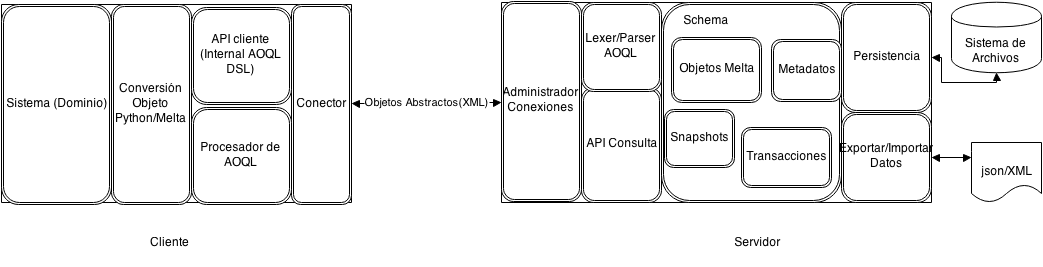
\includegraphics[width=19cm]{MeltaArchitecture}
\caption{Arquitectura General de Melta}
\label{fig:flies}
\end{figure*}

La comunicación entre el cliente y el servidor se realiza, en esta primera versión, serializando los objetos en XML, ya que permite de una manera simple intercambiar instrucciones entre estos a través de una red de comunicaciones. En una próxima versión se tratará de implementar un protocolo específico para serializar los objetos y operaciones que el servidor deberá manejar. Con respecto al XML, se presentó el problema de que pueda existir una posible colisión de nombres, por ejemplo, puede existir una Clase teléfono y una instancia de otra clase que tenga un estado teléfono. Para resolver esto, se utilizan los namespaces de XML \cite{xml:BHL06}, que proveen una manera de calificar nombres de atributos y elementos en documentos XML, asociandolos con namespaces identificados por referencias de \textit{Unified Resource Identifier} URI.

\section{Metamodelo de objetos}
\label{sec:metamodelo}
Este paper esta basado en gran parte en el paper de la OMG \cite{OMG:oodbs}, en el que se podrá hacer referencia para conocer más sobre esta sección. El modelo de objetos de Melta se diferencia del de los objetos nativos de Python, en disasociar los objetos con estado en un objeto compuesto, y sus estados como otros objetos atómicos, que pasarían a ser inmutables, o sea, ante el cambio, un objeto atómico no se actualiza sino que se crea uno nuevo y se desecha el anterior. Esto permitirá que pueda darse soporte en el futuro a objetos versionados, y facilita la restauración de un estado que esta asociado a una transacción ante un fallo de sincronización o \textit{rollback} de la transacción.
Dichos objetos, poseen un ID, único, generado en la creación inicial del objeto que se da cuando una instancia o valor es ingresado al \textit{schema}. Este ID, permitirá identificar unívocamente al objeto en el \textit{schema}, asi como la asociación entre ID de objeto de Python/Melta.
\\\\
\begin{figure}
\centering
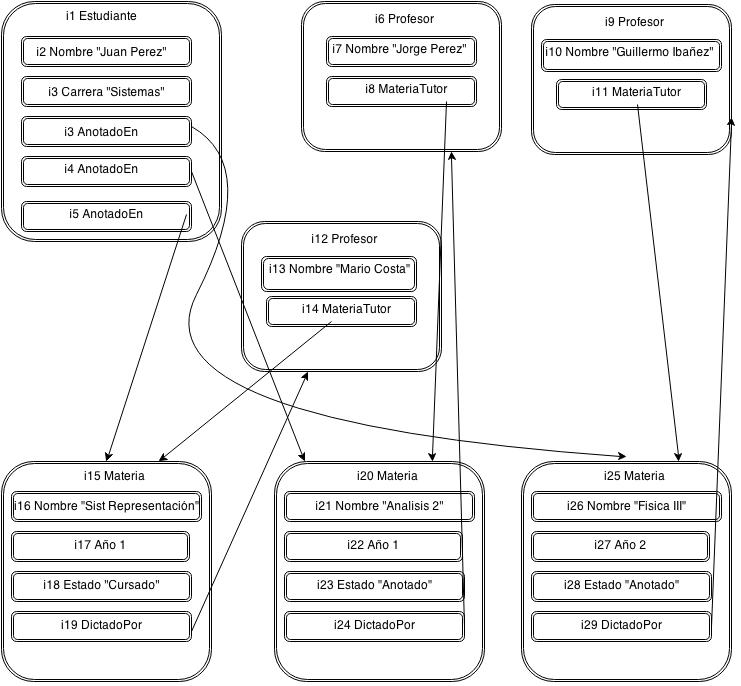
\includegraphics[scale=0.35]{modeloobjetos1}
\caption{Ejemplo de un schema de objetos en Melta.}
\label{melta:modeloObjetos}
\end{figure}

Los objetos que se encontrarán en el \textit{schema} o ecosistema de Melta en el servidor serán de estos tres tipos:
\begin{enumerate}
  \item \textbf{Objeto Atómico}: \textit{\textless i,n,v\textgreater} Son objetos, donde i es el ID del objeto, n es el nombre que tendrá el objeto, que será el nombre del atributo de la instancia de Python, y v el valor asociado al objeto. 
  \item \textbf{Objeto Compuesto}: \textit{\textless i,n,T\textgreater} Son objetos donde i es el ID, n el nombre de la instancia de Python y T, una lista de objetos atómicos o de referencia, que componen el objeto.
  \item \textbf{Objeto Referencia}: \textit{\textless i,n,r\textgreater} donde i es el ID del objeto, n el nombre de la instancia referida de Python y r, es el objeto Melta al que se hace referencia. Este tipo de objetos se generan, cuando una instancia tiene en su estado una referencia a otra instancia y representan este estado.
  \item \textbf{Objeto Clase}: \textit{\textless i,c,M,A\textgreater} donde i es el ID del objeto, c es el nombre de la Clase python, M es una lista de métodos que posee la clase y A es una lista ordenada con los ancestros de la clase que se representa en objeto. Las clases poseen invariantes, tales como los métodos de instancia que lo componen, el código que compone cada uno de los métodos, se serializa en un \textit{string} formateado, para respetar en el caso de Python, por ejemplo, la identación. Cuando se desee regenerar la clase nuevamente al levantar el sistema, se evaluarán estos \textit{strings} con el nombre del método almacenado y sus argumentos. Para los métodos de clase, se ha optado por tener un objeto que sea Metaclase.
  \item \textbf{Objeto MetaClase}:  \textit{\textless i,c,C,MC,A\textgreater} donde i es el ID del objeto, c el nombre de la Metaclase Python, C es el objeto clase de la base de datos asociada a dicho objeto Metaclase, MC es una lista de métodos de clase que suministrará al objeto clase C, y A es una lista de los ancestros del objeto Metaclase y son otros objetos Metaclase. Notese que la jerarquía de ancestros de C es la misma que la del objeto en cuestión, solo que el del este último son de objetos metaclase y no de objetos clase (Figura \ref{melta:Metaclase}).  
\end{enumerate}

\begin{figure}
\centering
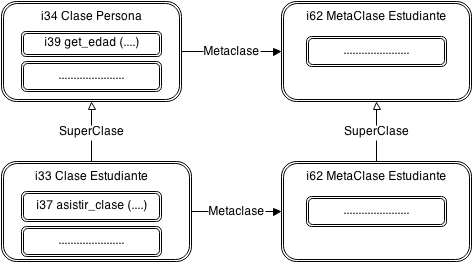
\includegraphics[scale=0.5]{MeltaMetaclase}
\caption{Ejemplo de la jerarquía de clases y metaclases.}
\label{melta:Metaclase}
\end{figure}


Como se menciono en la sección anterior, dichos objetos se encontrarán contenidos en el \textit{schema}, y estos representarán a aquellos objetos que se han recuperado de la base de datos y están en estado de transición durante el tiempo y que pueden variar de acuerdo al flujo del sistema de dominio (Figura \ref{melta:modeloObjetos}).
\\\\
Finalmente, todo objeto posee metadata asociado a el, en donde se define datos tales como la fecha de creación, modificación, si esta asociado a un \textit{schema}, la clase a la que pertenece, y si posee transacciones asociadas, entre otras cosas.

\subsection{Estructura del Schema}

El \textit{schema}, se compone por todos los objetos y clases que se hayan agregado a la base de datos, y además de eso, soporta lo que es la herencia dinámica. En el caso en el que tenemos un objeto de una clase que cambia luego su clase asociada por otro de la misma jerarquía, la base de datos debería evitar una reificación del objeto, descartando el viejo, y creando uno nuevo antes, a partir del estado del anterior, ya que se perdería la identidad del mismo. 
\\\\
\begin{figure}
\centering
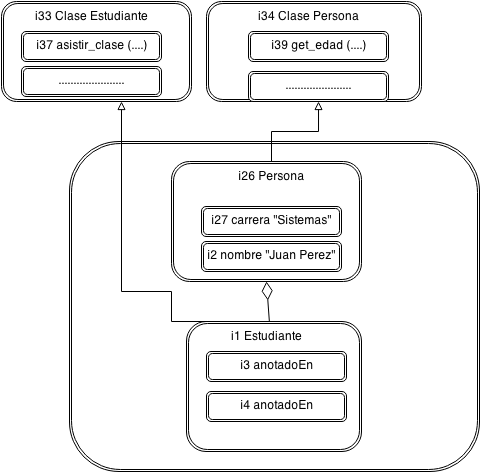
\includegraphics[scale=0.43]{MeltaHerenciaDinamica}
\caption{Herencia dinámica por medio de Roles.}
\label{melta:herenciaDinamica}
\end{figure}

Por ejemplo, si tenemos una clase Estudiante, que hereda de una clase Persona, y un objeto de este tipo (Estudiante); se tendría una instancia de este tipo con el estado propio de esta clase y otra instancia del tipo Persona con el estado que posee esta clase. En este caso el objeto del tipo Estudiante tendra una referencia al objeto de la clase Persona, que contiene parte de su estado. Esto rompe el principio de sustitución de Liskov, ya que no se podrá utilizar el objeto Estudiante, cuando se use en cambio el objeto Persona, ya que en este caso, Estudiante no sería más un subtipo de Persona.Esto se resuelve por lo explicado en \cite{OMG:oodbs}, mediante la implementación de roles, que hacen uso de la composición. Bajo este esquema, una aplicación puede definir subclases a partir de una clase, como en el caso de Estudiante-Persona, y cuando se necesite un objeto del rol Estudiante, el objeto, de la base de datos, de esta clase puede ser creado y ser asociado con el objeto de la superclase y ser disasociado, cuando ya no este actuando en este rol.
\\\\

\begin{figure*}
\centering
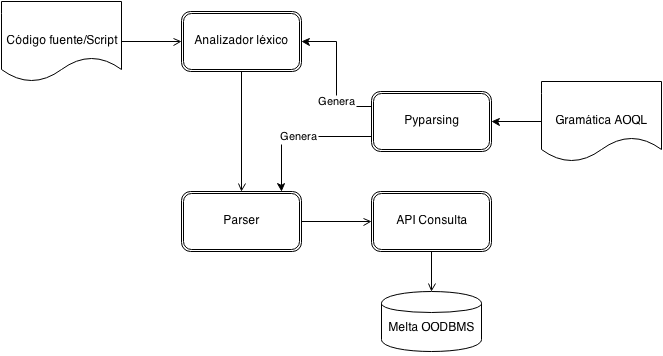
\includegraphics[scale=0.5]{MeltaAOQL}
\caption{Estructura del procesamiento del lenguaje de AOQL.}
\label{melta:aoql}
\end{figure*}

Ya explicada la herencia del \textit{schema}, se puede definir formalmente al mismo como una tupla \newline \textit{\textless O,C,R,CC,OC,OO \textgreater}, donde O representa a un hash o dicccionario de objetos, del tipo \{i : o\}, donde i es el ID del objeto, y o es la referencia del objeto en si mismo; C es una lista de las clases presentes en el ecosistema, R son los objetos raices del \textit{schema}, estos objetos, son aquellos que pertenecen a instancias de objetos Python. CC es una tabla de hash o dicccionario, del tipo \{c1 : A\}, que relaciona una clase \textit{c1} con su lista de ancestros \textit{A}. OC es un diccionario que relaciona lo que es un objeto con su clase. Notese que CC y OC, son datos que poseen estos objetos en sus respectivas estructuras de metadatos, y solo se vuelven a tener en el \textit{schema}, como tabla maestra. OO define una relación de lo que es la herencia dinámica entre objetos y roles. Por ejemplo si \{i1:i2\} 
\begin{math}
 \in
\end{math} OO, el objeto rol identificado como i1 esta heredado dinámicamente con el objeto identificado como i2. Un ejemplo de esto se ve en la Figura \ref{melta:herenciaDinamica}
\\\\
Con respecto a lo que es la actualización del sistema, el mismo se resolverá de acuerdo al mecanismo de transacciones, como se mecionó en la sección anterior. 

\section{Lenguaje de consulta AOQL}
\label{sec:aoql}
El lenguaje de consulta de AOQL (\textit{Abstract Object Query Language}), es vital para el acceso y persistencia de los datos que utilizará el sistema a lo largo de su ejecución. El mismo podrá ser utilizado en una consola, que actuará como cliente, como en el proyecto en el que se esta utilizando la base de datos. 
Este lenguaje de consulta definirá las operaciones necesarias para el uso de un cliente con la base de datos.
\\\\
Por otra parte el cliente no solo tendrá la posibilidad de comunicarse por medio de un lenguaje de consulta externo, sino que se ofrecerá la posibilidad de que puedan accederse por medio de sentencias en el mismo lenguaje de programación, que el sistema de dominio. De esta manera los programadores podrán hacer consultas sin tener que recurrrir a archivos externos donde esten las consultas, o a tener incluso las mismas mezcladas con el lenguaje de programación concreto del dominio. También se puede ver como no se necesitará de un parser previo para traducir la sintaxis del lenguaje AOQL, a las instrucciones Python propias de la API de consulta, en Python, que consultará a la base de datos.
\\\\
\label{table:gramatica}
\begin{table*}
\centering
\caption{Gramática de AOQL v1}
\begin{tabular}{|c|l|} \hline
Regla gramaticales&Nota\\ \hline
query ::= literal & lista L\\ \hline
query ::= name & lista N\\ \hline
query ::= operadorAlgUnario query& operadores algebráicos unarios\\ \hline
operadorAlgUnario ::= count \mid min \mid sum \mid max \mid - \mid sqrt \mid not \mid avg \mid & \\ \hline
query ::= query operadorAlgBinario query&\\ \hline
operadorAlgBinario ::== \mid< \mid > \mid + \mid - \mid * \mid / \mid and \mid or \mid intersect \mid ...&\\ \hline
query ::= query SinOperadorAlg query& Operador no algebráico.\\ \hline
SinOperadorAlg ::= where \mid . \mid join \mid \forall \mid \exists
query ::= \forall query query \mid \exists query query & Sintáxis alternativa de los identificadores. \\ \hline
query ::= query as name Name& Definición\\ \hline
query ::= query group as name& Agrupamiento\\ \hline
query ::= if query then query& Condicional\\ \hline
query ::= if query then query else query& Otra sintaxis de Condicional\\ \hline
querySeq ::= query \mid query, querySeq& Lista o secuencia de queries\\ \hline
query ::= struct( querySeq ) \mid (querySeq)& Structure constructor\\ \hline
query ::= list( ) \mid list( querySeq )& Constructor de Lista\\ \hline
query ::= set( ) \mid set( querySeq )& Constructor de Set\\ \hline
query ::= (role_name) query & \pbox{20cm}{Casteo dinámico para retornar \\ un rol en particular de un dataSet.} \\ \hline
query ::= query has role role_name& consulta de existencia del rol. \\ \hline
\hline\end{tabular}
\end{table*}


Se puede ver como ambas maneras de acceder a los datos, son coincidentes con lo que son los DSL's (\textit{Domain Specific Language}) externos e internos. En el que el lenguaje AOQL es un DSL externo, que requerirá una gramática asociada, ya que es independiente del lenguaje en el que se implementará la base de datos y el lenguaje en donde existirá el sistema que lo utilizará; y a su vez también tendrá un analizador léxico y un \textit{parser}, que puedan procesar el lenguaje y traducirlo a instrucciones de la API (figura \ref{melta:aoql}). En cambio las consultas hechas con comandos en un lenguaje de programación, en este caso será Python ya que se desarrollo el cliente en dicho lenguaje, directamente harán referencia a estas instrucciones de la API, y solo será un azucar sintáctico dicho DSL interno.
\\\\
En un futuro debería definirse un pequeño motor de optimización de consultas para minimizar la cantidad de operaciones hacia el servidor y de esta manera tener un menor tiempo de espera, en obtener datos o resultados por parte del cliente.

\subsection{Gramática del lenguaje AOQL}

El lenguaje de AOQL, en su primera versión estará conformada por la gramática descripta en la tabla 1.
\\\\
Dicha tabla estaba basada en el trabajo en \cite{OMG:oodbs}, con algunas pequeñas modificaciones. En el futuro, se podría pensar una extensión de los tipos de colecciones para soportar otros lenguajes de programación que hagan uso de este motor. En cuanto a la implementación, se implemento el lenguaje utilizando una herramienta que permite generar un analizador léxico y un \textit{parser} a partir de la gramática definida en la tabla. Luego de eso, se armo un intérprete directo que hace uso de la API de consulta contra la base de datos.


\section{Persistencia}
\label{sec:persistencia}
Melta posee un modulo de persistencia en donde se almacenarán físicamente los objetos pertenecientes al \textit{schema}, una vez que se haya hecho un \textit{commit} en laa transacción. En la primera versión solamente se persistirán los cambios detectados en el sistema hacia el \textit{schema}, solo cuando esto suceda. 
\\\\
Los objetos en Melta, estan identificados por un ID único de 128bits de longitud, generado cuando se introduce un objeto en la base de datos, y el mismo tiene un formato similar al de UUID, definido en la RFC4122 \ref{UUID:Leach}. Este identificador unívoco se utilizará en el archivo donde se almacenarán a aquellos objetos que no estén siendo utilizados durante la ejecución. Cuando se solicite un objeto, por parte de un cliente, que no exista actualmente en el schema, se procederá a leerlo del archivo en donde esta almacenado, y un módulo de extracción convertirá el objeto serializado en formato Melta, asimismo, se extraerá la metadata del mismo que tabien ha sido serializado. Cuando se reconstruye el objeto, se chequeará si la clase o rol que tiene asociado actualmente existe en el \textit{schema}, si no existe se traerá el mismo también.
\\\\
Con respecto al formato del archivo, actualmente esta en desarrollo, pero se tendrá probablemente una primera versión del mismo, con una arquitectura, en la que la persistencia de un \textit{schema}, se haga en dos archivos separados, el primero será de extensión .mlt, donde se almacenarán todos los objetos pertenecientes al \textit{schema}, una vez que se transaccione, el mismo estará compuesto por una cabecera de 8192 bytes, que contendrá una \textit{binary signature}, que procurará la integridad de los datos a cierto punto (esto depende del algoritmo que se emplee para este propósito), un número de versión, la metadata propia del \textit{schema}, cantidad de objetos persistidos, el tamaño del archivo total, una lista de punteros libres, y el puntero inicial donde comienza el primer objeto. Luego se tendrá un directorio, donde estará el puntero de cada uno de los objetos que conforman el archivo. El mismo es de una longitud fija de 8192 bytes, y en caso de que se supere dicho límite, siempre tendrá una referencia al próximo bloque del directorio, y de esta manera, se comporta como una lista secuencial de bloques.
\\\\
Luego del directorio se tendrán los objetos, de longitud variable, de acuerdo a lo que ocupen, cuando se agrega un nuevo objeto se agrega al final del archivo, y cuando se elimina uno, se libera el bloque del disco, y se agrega el puntero a la lista de punteros libres. El problema que existe es análogo al que sucede con un asignador de memoria, en el que habrá fragmentación a medida que pase el tiempo, para remediar esto, en primera medida, cada X (este valor es configurable) veces que se monte el filesystem, cuando se inicializa la base de datos, se compactará el archivo y se actualizará el directorio. Una mejora a esto sería que en vez de agregar siempre al final se tenga un algoritmo de first-fit, y de esta manera se reduzca el espacio libre fragmentado, sin embargo, se deberá hacer una compactación luego de un tiempo. 
\\\\
El segundo archivo contendrá los datos de indexación de los objetos, y este archivo se levantará en su totalidad cuando se inicialice el motor de base de datos, su objetivo es obtener rápidamente los objetos a restaurar por clase, y la reindexación la manejará automáticamente el modulo de persistencia y recuperación. Este archivo solo se persistirá cuando se guardan los cambios en la base de datos, y al estar levantado todo el índice en memoria, no existirá fragmentación.
\\\\
Finalmente cuando una transacción global sea exitosa, se guardará los cambios en el \textit{schema}, consecuentemente hay una manera de decir al sistema de que se desean persistir en disco lo que existe actualmente en el \textit{schema}, y es mediante un comando llamado snapshopt, que persistirá los cambios en el disco. 

\section{Transacciones y Concurrencia}
\label{sec:tran}
Melta soporta modificaciones concurrentes de objetos, por varios clientes que esten conectado al servidor, toda modficiación, del lado del cliente debe estar enmarcado en una transacción, esto provee dos características importantes:

\begin{itemize}
\item \textbf{Atomicidad}: Las transacciones son exitosas o falla, y al ser transacciones, no hay estado que se mantenga hasta que se haga \textit{commit} a una transacción.
\item \textbf{Control de Concurrencia}: las transacciones se ejecutan como si tuviesen acceso exlusivo a los datos, de esta manera, multiples transacciones pueden correr concurrentemente y de esta manera la lógica de la aplicacion no tiene que tomar en cuenta el acceso concurrente.
\end{itemize}

Las transacciones utilizan el principio de \textit{Optimistic Concurrency Control}, mediante un timestamp. Los cambios que se hacen a uno o más objetos mientras los cambios no esten aplicados, mediante un \textit{commit}, son realizado de manera independiente y del lado del cliente, que mantendrá sus objetos modificados en una cache, y de esta manera no tiene que ser bloqueados, los cambios recien se sincronizarán cuando el cliente haga un \textit{commit} explicito. Solo se permite que una transacción aplique los cambios en un momento determinado. Si hay dos threads, o clientes, que modifican un el mismo objeto, uno de ellos aplicará los cambios primero. Cuando el segundo aplique los cambios, el cambio que aplique será inválido y se le retornará una excepción al mismo. El dominio o aplicación debería atrapar esta excepción y ejecutar de nuevo la aplicación de los cambios, cuando esto suceda, los estados de los objetos afectados, reflejan cambios hechos por las transacciones ya exitosas en el servidor.

\section{Conclusiones}
\label{sec:conc}
Si bien este paper es una versión temprana de un prototipo de una base orientada a objetos, en esta primera versión se definió una primera aproximación de una arquitectura para un model cliente/servidor básico. Los próximos objetivos, para tener un prototipo más completo, son los siguientes:

\begin{itemize}
\item Objetos versionados.
\item Replicación.
\item Bases de datos federadas.
\item Optimización del Motor y de sentencias AOQL.
\item Acceso cruzado a otras bases de datos orientas a objetos.
\item Proponer un protocolo para comunicación de objetos y operaciones entre cliente/servidor.
\item Tolerancia a fallos, por interrupción del servicio causado por fallas electricas o de red.
\end{itemize}
%\end{document}  % This is where a 'short' article might terminate

Actualmente se esta desarrollando una implementación de este protoripo, como se mencionó en la introducción, y el objetivo es implementar la arquitectura propuesta en este documento. Los siguientes pasos involucrarían la optimización del motor y de testear el mismo con una mayor carga de datos a fin de evaluar si es viable el uso de este motor en ambientes productivos. 
Si bien algunas de las partes, como el metamodelo son basadas fuertemente en \cite{OMG:oodbs}, se hicieron algunas modificaciones sobre este, y se diseño una arquitectura simple para una primera versión de este motor de base de datos. 


% ensure same length columns on last page (might need two sub-sequent latex runs)
\balance

%ACKNOWLEDGMENTS are optional
\section{Agradecimientos}
Agradecimientos en especial a la OMG, por su propuesta de un nuevo estandar, que me dio el interés para investigar y desarrollar este prototípo en esta tecnología emergente.

\newpage
\nocite{*} 
% The following two commands are all you need in the
% initial runs of your .tex file to
% produce the bibliography for the citations in your paper.
\bibliographystyle{abbrv}
\bibliography{melta_blib}  % vldb_sample.bib is the name of the Bibliography in this case
% You must have a proper ".bib" file
%  and remember to run:
% latex bibtex latex latex
% to resolve all references

%APPENDIX is optional.
% ****************** APPENDIX **************************************
% Example of an appendix; typically would start on a new page
%pagebreak

%\begin{appendix}

%\end{appendix}



\end{document}
